% AUTO-GENERATED VECTOR PLOTS FROM results/metrics.json

\begin{figure}[t]
  \centering
  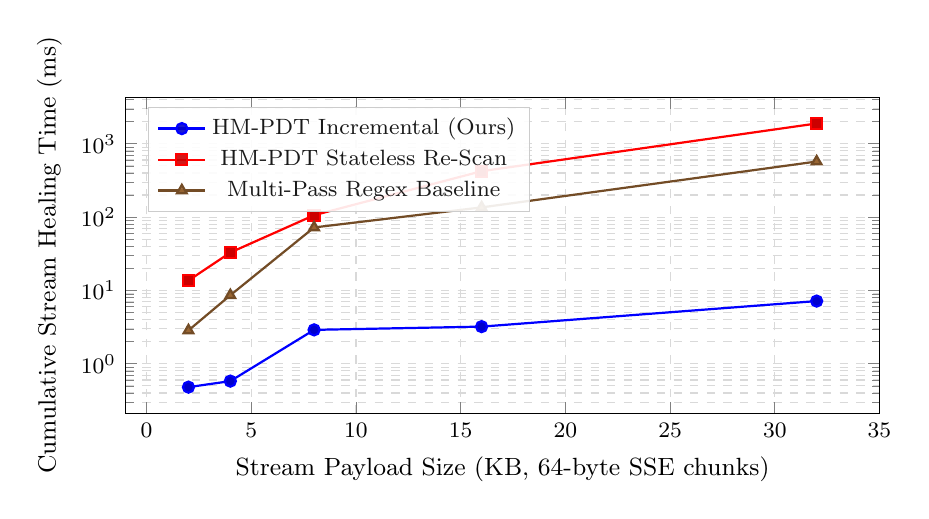
\begin{tikzpicture}
    \begin{axis}[
      width=0.92\columnwidth,
      height=5.6cm,
      xlabel={Stream Payload Size (KB, 64-byte SSE chunks)},
      ylabel={Cumulative Stream Healing Time (ms)},
      ymode=log,
      grid=both,
      grid style={dashed,gray!30},
      legend pos=north west,
      legend style={font=\footnotesize, draw=gray!40, fill=white, fill opacity=0.9},
      tick label style={font=\footnotesize},
      label style={font=\small}
    ]
      \addplot+[thick, mark=*] coordinates { (2,0.48) (4,0.58) (8,2.9) (16,3.21) (32,7.16) };
      \addlegendentry{HM-PDT Incremental (Ours)}
      \addplot+[thick, mark=square*] coordinates { (2,13.64) (4,32.88) (8,106.13) (16,422.98) (32,1891.76) };
      \addlegendentry{HM-PDT Stateless Re-Scan}
      \addplot+[thick, mark=triangle*] coordinates { (2,2.85) (4,8.6) (8,72.28) (16,135.64) (32,572.61) };
      \addlegendentry{Multi-Pass Regex Baseline}
    \end{axis}
  \end{tikzpicture}
  \caption{Empirical asymptotic scaling from 2 KB to 32 KB streaming outputs (log-scale y-axis). Stateless full-buffer re-scanning and multi-pass regex pipelines incur quadratic cumulative latency growth, whereas our Incremental HM-PDT maintains linear cumulative scaling.}
  \label{fig:scaling_complexity}
\end{figure}
